
%%%%%%%%%%%%%%%%%%%%%%%%%%%%%%%%%%%%%%%%%%%%%%%%%%%%%%%%%%%%%%%%%%%%%%%
%% $Id: report.tex,v 1.5 2005/02/09 21:06:42 lindstrm Exp $
%%%%%%%%%%%%%%%%%%%%%%%%%%%%%%%%%%%%%%%%%%%%%%%%%%%%%%%%%%%%%%%%%%%%%%%
%% costhesis usage example
%% modified and added to by GQMJr
%%%%%%%%%%%%%%%%%%%%%%%%%%%%%%%%%%%%%%%%%%%%%%%%%%%%%%%%%%%%%%%%%%%%%%%
%
% The costhesis package accepts the following options
%
%   Document types:
%     msc               - Master Thesis
%     bsc		- Kandidate Thesis
%
%   Layout options:
%
%   Other options:
%     blank             - Removes pagenumbers and headers from empty pages
%     blankmsg          - Prints a message of intent on empty pages
%     scheader          - Typeset headers in SMALL CAPS shape (default)
%     slheader          - Typeset headers in slanted shape 
%
%
%
%

\documentclass[12pt,a4paper,twoside,openright]{book}
%%\documentclass[12pt,a4paper,twoside,openright]{memoir}

\usepackage[msc,blankmsg]{costhesis}
%\usepackage[T1]{fontenc}
%%\usepackage{pslatex}
\renewcommand{\rmdefault}{ptm} 
\usepackage{mathptmx}
\usepackage[scaled=.90]{helvet}
\usepackage{courier}
%
\usepackage{bookmark}


%% ------------------------------------------------------------------
% Equation Packages
%% ------------------------------------------------------------------


\usepackage{times,amsmath,epsfig}
\usepackage[utf8]{inputenc}
\usepackage[usenames,dvipsnames]{color}
\usepackage{amssymb}

\let\labelindent\relax

\usepackage{graphicx}
\usepackage{caption}
\usepackage{hyperref}
\graphicspath{ {images/} }
\usepackage[many]{tcolorbox}
\usepackage{subcaption}
\usepackage{balance}  % for  \balance command ON LAST PAGE  (only there!)
\usepackage{pdfpages}
\usepackage{fancyhdr}
\usepackage{exscale}
\usepackage{booktabs}
\usepackage{multicol}
\usepackage{multirow}
\usepackage{amsfonts}
\usepackage{amssymb}
\usepackage{ntheorem}
\usepackage{paralist}
\usepackage{verbatim}
\usepackage{color}
\usepackage{hyperref}
\usepackage{enumitem}
\usepackage{listings}      % source code
\usepackage{algorithm}
\usepackage{algorithmicx}  % pseudo code (1/2)
\usepackage[noend]{algpseudocode} % pseudo code (2/2)
\usepackage{setspace}
\usepackage{array}
\usepackage{relsize}
\usepackage{diagbox}
\usepackage{listings}


\DeclareMathOperator{\union}{\mathtt{union}}
\providecommand{\myfloor}[1]{\left \lfloor #1 \right \rfloor}

%%%%%%TRIGGER
\algblockdefx[TriggerS]{TriggerS}{EndTriggerS}[2][event]
  {\textbf{trigger} $\langle #1 \rangle$;}

%No extra line - TriggerS 
\makeatletter
\ifthenelse{\equal{\ALG@noend}{t}}%
  {\algtext*{EndTriggerS}}
  {}%
\makeatother

\algblockdefx[Trigger]{Trigger}{EndTrigger}[2][event]
  {\textbf{trigger} $\langle#1$ $\mid$ $#2\rangle$;}

%No extra line - Trigger  
\makeatletter
\ifthenelse{\equal{\ALG@noend}{t}}%
  {\algtext*{EndTrigger}}
  {}%
\makeatother

%%%%%%FOR EACH
\algblockdefx[ForEach]{ForEach}{EndForEach}[2][collection]
   {\textbf{ for each } $#1$ \textbf{as} $#2$}

%No extra line - ForEach
\makeatletter
\ifthenelse{\equal{\ALG@noend}{t}}%
  {\algtext*{EndForEach}}
  {}%
\makeatother

%%%%%%UPON
\algblockdefx[UponEvent]{Upon}{EndUpon}[2][event]
  {\textbf{upon event} $\langle#1$ $\mid$ \emph{#2}$\rangle$ \textbf{do} }

\algblockdefx[UponEventS]{UponS}{EndUponS}[2][event]
  {\textbf{upon event} $\langle#1\rangle$ \textbf{do} }




%%----------------------------------------------------------------------------
%%   pcap2tex stuff
%%----------------------------------------------------------------------------
% \usepackage[dvipsnames*,svgnames]{xcolor} %% For extended colors
% \usepackage{tikz}
 \usetikzlibrary{arrows,decorations.pathmorphing,backgrounds,fit,positioning,calc,shapes}
% \usepackage{pgfmath}	% --math engine
%%----------------------------------------------------------------------------
%\usepackage[latin1]{inputenc}
\usepackage[utf8]{inputenc} % inputenc allows the user to input accented characters directly from the keyboard
\usepackage[swedish,english]{babel}
\usepackage{rotating}		 %% For text rotating
\usepackage{array}			 %% For table wrapping
\usepackage{graphicx}	 %% Support for images
\usepackage{float}			 %% Suppor for more flexible floating box positioning
\usepackage{color}           %% Support for colour 
\usepackage{mdwlist}
\usepackage{setspace}    %% For fine-grained control over line spacing
\usepackage{listings}		%% For source code listing
\usepackage{bytefield}    %% For packet drawings
\usepackage{tabularx}		%% For simple table stretching
\usepackage{multirow}	%% Support for multirow colums in tables
\usepackage{dcolumn}	%% Support for decimal point alignment in tables
\usepackage{url}	%% Support for breaking URLs
\usepackage[perpage,para,symbol]{footmisc} %% use symbols to ``number'' footnotes and reset which symbol is used first on each page

%%\usepackage{pygmentize}  %% required to use minted -- see python-pygments - Pygments is a Syntax Highlighting Package written in Python
%\usepackage[outputdir=.texpadtmp]{minted}
\usepackage{minted}		%% For source code highlighting
\usemintedstyle{borland}


\usepackage{hyperref}		
\usepackage[all]{hypcap}	 %% Prevents an issue related to hyperref and caption linking
%% setup hyperref to use the darkblue color on links
\hypersetup{colorlinks,breaklinks,
            linkcolor=darkblue,urlcolor=darkblue,
            anchorcolor=darkblue,citecolor=darkblue}


%% Some definitions of used colors
\definecolor{darkblue}{rgb}{0.0,0.0,0.3} %% define a color called darkblue
\definecolor{darkred}{rgb}{0.4,0.0,0.0}
\definecolor{red}{rgb}{0.7,0.0,0.0}
\definecolor{lightgrey}{rgb}{0.8,0.8,0.8} 
\definecolor{grey}{rgb}{0.6,0.6,0.6}
\definecolor{darkgrey}{rgb}{0.4,0.4,0.4}
%% Reduce hyphenation as much as possible
\hyphenpenalty=15000 
\tolerance=1000

%% useful redefinitions to use with tables
\newcommand{\rr}{\raggedright} %% raggedright command redefinition
\newcommand{\rl}{\raggedleft} %% raggedleft command redefinition
\newcommand{\tn}{\tabularnewline} %% tabularnewline command redefinition

%% definition of new command for bytefield package
\newcommand{\colorbitbox}[3]{%
	\rlap{\bitbox{#2}{\color{#1}\rule{\width}{\height}}}%
	\bitbox{#2}{#3}}

%% command to ease switching to red color text
\newcommand{\red}{\color{red}}
%%redefinition of paragraph command to insert a breakline after it
\makeatletter
\renewcommand\paragraph{\@startsection{paragraph}{4}{\z@}%
  {-3.25ex\@plus -1ex \@minus -.2ex}%
  {1.5ex \@plus .2ex}%
  {\normalfont\normalsize\bfseries}}
\makeatother

%%redefinition of subparagraph command to insert a breakline after it
\makeatletter
\renewcommand\subparagraph{\@startsection{subparagraph}{5}{\z@}%
  {-3.25ex\@plus -1ex \@minus -.2ex}%
  {1.5ex \@plus .2ex}%
  {\normalfont\normalsize\bfseries}}
\makeatother

\setcounter{tocdepth}{3}	%% 3 depth levels in TOC
\setcounter{secnumdepth}{5} %% 3 sectioning levels. WARNING: command \mainmatter resets this field to its default value!!!
%%%%%%%%%%%%%%%%%%%%%%%%%%%%%%%%%%%%%%%%%%%%%%%%%%%%%%%%%%%%%%%%%%%%
%% End of preamble
%%%%%%%%%%%%%%%%%%%%%%%%%%%%%%%%%%%%%%%%%%%%%%%%%%%%%%%%%%%%%%%%%%%%

\iauthor{Abhimanyu Babbar}
\ititle{Peer to Peer Search Protocol}
\isubtitle{Network Partition Aware Decentralized Search}
\idate{2015}{June}{12}
\examinername{Professor Seif Haridi}

\setlength{\headheight}{15pt}
\begin{document}

\frontmatter
\selectlanguage{english}
\begin{abstract}
\label{sec:abstract}
\setcounter{page}{1}


Your abstract here.

\end{abstract}
%%\clearpage
\selectlanguage{swedish}
%%\chapter*{Sammanfattning}
\begin{abstract}
\label{sec:swedish_abstract}


IETF xxxx Arbetsgruppen har definierat 
\end{abstract}

\selectlanguage{english}
\begin{acknowledgements}
I would like to thank my examiner \textit{Seif Haridi} and my supervisor \textit{Dr Jim Dowling} for providing me the opportunity to perform this research and guiding me through it.
\par I would also like to extend my gratitude towards \textit{Alexandru - Adrian Ormenisan} for providing a constant stream of inputs, insight and feedback regarding the ideas during the research.

\end{acknowledgements}

\selectlanguage{english}
\tableofcontents

\listoffigures

\listoftables

%% add a list of listing if and listings are used
\listoflistings

% \begin{notations}
% \end{notations}

\renewcommand\abbreviationsname{List of Acronyms and Abbreviations}
\begin{abbreviations}
\label{list-of-acronyms-and-abbreviations}

This document requires readers to be familiar with terms and concepts described in \mbox{RFC~1235} \cite{john_ioannidis_coherent_1991}. For clarity we summarize some of these terms and give a short description of them before presenting them in next sections.

\begin{basedescript}{\desclabelstyle{\pushlabel}\desclabelwidth{10em}}
\item[IPv4]					Internet Protocol version 4 (RFC~791 \cite{postel_internet_1981})
\item[IPv6]					Internet Protocol version 6 (RFC~2460 \cite{deering_internet_1998})
\end{basedescript}
\end{abbreviations}

\mainmatter
\setcounter{secnumdepth}{5} 
\chapter{Introduction}
\label{chap:introduction}
%% Longer problem statement
%% General introduction to the area



\section{Problem description}
\label{sec:problem_description}




\section{Problem context}
\label{sec:problem_context}



\section{Structure of this thesis}
\label{sec:thesis_structure}

Chapter \ref{chap:introduction} describes the problem and its context.
Chapter \ref{chap:background} provides the background necessary to understand the
problem and the specific knowledge that the reader will need to understand the
rest of this thesis. Following this Chapter \ref{chap:method} describes the
goals, metrics, and solution proposed in this thesis project. The solution is
analyzed and evalued in Chapter \ref{chap:analysis}. Finally, Chapter
\ref{chap:conclusion} offers some conclusions and suggests future work.


\chapter{Background}
\label{chap:background}

%%    What does a reader (another x student -- where x is your study line) need to know to understand your report?
%%    What have others already done?
This section will present a brief introduction about the full text search and distributed databases. In addition to this, the decentralized search prototype is developed in Kompics[reference], so we will also be providing a brief introduction about the same. In addition to this, we will also be mentioning Git Merge protocols which is used as a motivation for the potential Network Partition Merge Strategy.


\section{Apache Lucene}

Apache Lucene [reference] is a robust and an extremely fast Java Library which was written by Doug Cutting in the year 1999. It is mainly used for \textit{full text searching}. Lucene has been thoroughly tested and is used by companies like Twitter[reference] and ElasticSearch[reference] to provide with full text search. At the core of Lucene is concept of Index containing Documents. Documents are mainly containers of information that needs to be indexed. Its the responsibility of the application to construct the Document by adding the data as fields in it. The ability to treat Documents as collection of fields with text is main reason behind the powerful nature of Lucene. This allows user to index files of any format like PDF, HTML, Excel etc. 

\section{Kompics}
Kompics[reference] is an \textit{Asynchronous Message Passing} framework based on Component Model. The main purpose of Kompics is to simplify the development of complex distributed applications by leveraging multi-core machines and providing a robust simulation framework with capability of providing reproducible results. 
\par As mentioned above, Kompics is based on a Component Model which is mainly a reactive state machine. These components execute concurrently and communicate asynchronously by message passing. These messages are known as \textit{Events} which are immutable typed objects. The information contained in these events is in form of attributes. Each component usually exposes an interface to other components known as \textit{Port}. These ports define the events that can pass through them and therefore act as filters by allowing specific events. In order to send an event between components, we need a communication medium or a link. This abstraction is known as \textit{Channel}. A channel connect ports of complimentary nature. The events sent over the channel are transferred and received by other component in FIFO order. In addition to this, each Component contains \textit{Handlers} which are first class procedures. Each handler is responsible for handling a particular type of event and gets executed when the component receives that event. The handler has capability to in turn trigger new events on other components. 


\section{Google Search}
Nowadays, search on web is synonymous with Google Search. It has a robust network of hardware devices and in house software that allows it to handle millions of search requests everyday. A closer look at the software infrastructure[reference gs] reveals the presence of data structure known as \textit{Inverted Index} used for indexing the documents. The index containing the documents is divided into many pieces known as shards which are distributed and handled by multiple machines. This greatly helps in improving the search response by parallelizing the requests to these multiple shards which contain a subset of data. 
\par The search request is initially handled by a DNS based load balancer which redirects the query to a nearby cluster. The query is then processed by the cluster by sending the request to multiple shards in parallel. Inside each shard a dedicated machine is responsible for handling queries. In first stage of the request, a list of doc id's matching the request is returned. The actual documents relating to these id's are fetched from the machines in the next stage. The results are sorted and returned back to the requesting node.


\section{Git Merge}
In this section, we will be providing a brief introduction about Git and the strategies for \textit{Branching and Merging} used in it[reference]. Git is a popular distributed version control system used to record changes made to a particular file over time[reference version control]. Git is advancement over the previous centralized version control systems like VCS[reference] and SVN[reference] in sense that users unlike checking out particular files of the project located in centralized server simply checkout the whole project. This prevents a single point of failure as the server hosting the project in case of SVN could simply crash and the users are left with snapshots of specific checked out file. Git prevents it by \textit{cloning} whole project on to the user local directory. In addition to this, Git store the data and subsequent changes as separate snapshots of files in the projects which is in contrast to the process of storing base files with snapshots of incremental changes made to that file. This feature helps in committing changes to the git locally instead of trying to reach server everytime. Thus user can bundle the commits locally in case of absence of network and push them once available.
\par The feature of git that makes it stand apart from its predecessors is the model used for branching and merging back. Git makes it very easy for the user to create different branches of the same project and work independently on them. In git, each commit containing changes to the files also has a unique value associated with it. In addition to this, it also has a reference to the previous commit. In this it allows user to work on a separate branch and allow it to make several commit. When the user decides to merge the data back in main branch, git looks at the \textit{HEAD} of the two branches and calculate the common ancestor. The git then calculates the changes made in both branches since the common ancestor and uses an intelligent strategy to merge and apply changes to a resultant branch. 


\section{CAP Theorem}
Eric Brewer in the year 2000 put forward his opinion that in a distributed system we cannot achieve both \textit{Consistency} and \textit{Availability} during the event of \textit{Network Partitioning}. A distributed system that spans over thousands of machine usually see switches failing and communication between the nodes being interrupted. Therefore a set of nodes is whole system becomes unreachable resulting in network partitioning. At this stage, the application needs to decide based on the requirements to either provide \textit{Consistency} in sense that allow all user to read the previous written writes or focus on \textit{Availability} by providing the read and write capability in the system even in event of Network Partitioning.


\chapter{Related Work}
\label{sec:related_work}



\section{Cassandra}
Cassandra[reference] is a highly available distributed key value system deployed for managing backened services in Facebook. The system is developed for storing highly structured values. The system offers a simple API involving \textit{get, insert} and \textit{delete} operations.
\par The system uses consistent hashing[reference] to identify the location of the node on the ring and data keys. A node is responsible for storing the keys which lie between the node and the successor. In order to prevent single point of failure, the keys are replicated over the \textit{N -1} successor nodes. Based on different policies for data replication, the other nodes used for replication of the key are selected. In addition to this, in case the load on a particular node increases, the system boots up separate light weight node and inject the node between the highly loaded node and its successor. As the new node joins, it becomes responsible for the keys between it and the successor.

\section{Dynamo}
Dynamo[reference] is Amazon's highly available key value store. The system is designed to focus on and provide availability even in event of network partition. The system's API provides a simple \textit{get(key)} and \textit{put(key, value)} functionality. 

\par In order to provide the always write functionality, the system extensively makes use of the object versioning. Even in the event of network partitioning, the users can write to the system. The conflicts that arise after the partition merge are sometimes offloaded to user for resolving. The system also makes use of Consistent Hashing to determine the location of the nodes on the ring and the position of the key for the data to be stored. The node is responsible keys lying between himself and its successor. The system realizes the bias introduced by the consistent hash in terms of uneven load on different nodes. In order to resolve this, it uses a modified version of consistent hash in which the a node is assigned to multiple positions in the ring. In this way, the node becomes host for multiple regions in the ring.
\par In order to search for a particular key, the consistent hash reveals the position of the key on the ring. The request is then routed to the node responsible the key. 


\section{ElasticSearch and Solr}

\chapter{Method}
\label{chap:method}

%% What are your goals? (What should you be able to do as a result of your solution - which couldn't be done well before you started?)
%%  What you are going to do? Why?

\chapter{Analysis}
\label{chap:analysis}

%% How you are going to evaluate what you have done?
%% Analysis of your data and proposed solution
%% Does this meet the goals which you had when you started?



\chapter{Design and Architecture}
\label{sec:design}

\section{System Model}

\begin{itemize}

\item \textit{Peers}: The system is composed of peers which basically are processes executed by the clients. The clients join the system by bootstrapping themselves with the already present peers in the system. The peers follow the Crash/ Stop process [ref] i.e a peer upon failure crashes and stops all communication with the other nodes. Once the node has failed that node never comes up. 


\item \textit{Communication Links}: As part of system design we assume the communication link to be fair-loss links[reference]. Therefore, the network only transfers the messages that are sent from the application and cannot create the messages on its own. In addition to this, we assume the network to be partially synchronous meaning there are times during which the network might being asynchronous and drop messages but eventually the network will become synchronous with upper bounds on the message transmission time.

\item \textit{Overlay Network}: The system is built upon Gradient [reference] which constructs an overlay based on the preference function. The preference function used for the application will be explained later in detail but in general it helps to identify the ranking of node as compared to others. The Gradient in turn is built upon a peer sampling service which provides random samples from the application to the Gradient component.

\end{itemize}



\section{Overlay Network}
In this section, we will briefly discuss about the overlay network over which the system is built. The two main components used to construct the overlay network are as follows: 

\subsection{Gossiping}
The system runs over a simple gossiping protocol which forms the basis for the overlay topology management. The gossiping protocol is inspired from the Peer Sampling Service[reference] which provides each peer with a list of other peers in the system which is a uniform random sample of all the peers. The peers then exchange information with other peer selected from the list based on some well defined policies. The gossiping protocol are generally used in information dissemination, scalability, churn management etc.


\subsection{Structured Overlay}

Gradient[reference] which is a class of structured P2P overlays forms the basis for the overlay of the system. In this overlay, the nodes select there neighbors based on a well defined preference function. The preference function used in case of the prototype developed as part of thesis is explained in detail in the later sections [Mention Section]. The uniform random sample from the \textit{Peer Sampling Service} is fed into the Gradient. Based on the preference function the node select the best peer to exchange information with. In this way, the structured overlay is constructed and maintained.


\section{Architecture}

The actual structure of a distirbuted search engine is usually complex. It involves modules for the request routing, leader election, overlay management, load balancing and searching the data.Figure \ref{fig:architecture} depicts a high level view of the system involving routing requests to specific shards based on the category. In this section we will look at the 

\begin{figure}[h]
	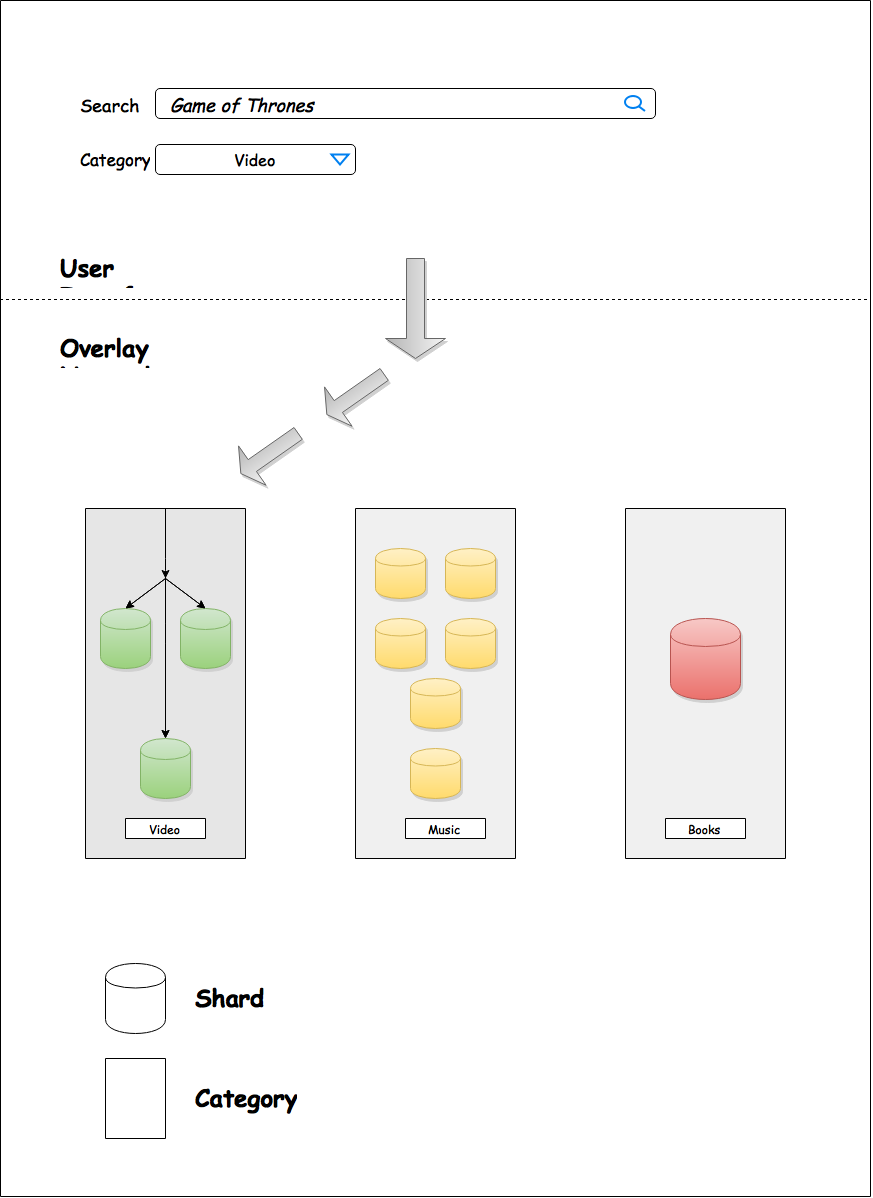
\includegraphics[width=10cm, height=12cm]{architecture}
	\centering
	\caption{Architectural Overview}
	\label{fig:architecture}
\end{figure}

\subsection{Leader Election Protocol}

In context of distributed systems various leader election protocols have been discussed {several references}. Election of leader for a group of nodes in the system typically requires all the nodes to agree upon the leader. Once the leader gets elected, it coordinates between the nodes and helps the group to move forward. 
\par As mentioned above, all the nodes usually need to know about the node that would be elected as leader but in case of large scale system it would usually result in huge traffic in the system. As part of this research, we introduced a weaker form of leader election protocol known as \textit{Leader Selection}. As part of this protocol, we select a group of \textit{top K} nodes in the system. The node which has the highest utility among the K members tries to assert itself as the leader. Figure \ref{fig:p-arrange} provides a general overview of the system in which the top nodes are located at the center and as we go towards the leaf the utility decreases depicted with the color gradient. The node, in order to become the leader asks for promises from the other nodes in the selected group. In case, the nodes see anybody above the node rejects the promise. The requesting only moves to the commit phase after receiving promises from all the nodes in the group. In case any one of them rejects, the node resets the convergence counter and waits for the system to stabalize again. 

\par In order to better understand the mechanism, we need to look at the overlay over which the system is built. We use the Gradient topology, which is a class of P2P topology in which the nodes in the systems organize themselves in the network in such a way that the nodes with the highest utility  are concentrated at the center of the network and the nodes with low utility lies on the outer edges of the network. We use a \textit{preference function}, according to which nodes have a higher preference to form connections with the nodes which have utility higher but closer to itself with higher probability. In this way the nodes arrange themselves in the system. In addition to this, every node runs a convergence function in which it tries to calculate a percentage change in the number of neighbors. In case the change is greater than a predefined threshold \textit{D}, the node resets the convergence counter. On the other hand, if the change is below the threshold the node increments the counter. 
\par The node only tries to assert itself the leader, when the convergence counter has reached a certain value and the node based on its own utility sees no other node above it. It is then the node starts the promise round with the other K nodes. This process of determining if self node is a leader is carried out by every node in every shard in the system. Eventually the leader gets elected for every shard. In addition to leader, every shard also has a follower group selected by the leader itself. The purpose of the follower group is to help the leader with the replication of the commands and the steps taken by the leader. In case the leader dies, the next higher node usually from the follower group takes over the leadership for that shard. The main functionality of the members of the followers group is as follows:


\begin{enumerate}

\item Reject all promises in case the node has already promised or is a part of follower group.

\item Accept a promise in case the node doesn't see anybody above the requesting node in terms of utility.

\item Expire a promise in case the commit message is not received before the timeout for a specific promise.

\end{enumerate}


As part of the leader selection mechanism, we try to elect a leader as soon as possible. In a very dynamic system where nodes can join and leave the system, it is very much possible that a better node comes along and try to assert itself as a leader thus violating the safety condition of having only a single leader per shard in the system. In order to prevent this, when a node gets elected as the leader, it along with the chosen follower group, artificially augments the utility by switching on the leader memebership check. This check places the group at the center of the shard. In this way when a better node comes along, it cannot instantaneously start the election protoco because it's self membership check is switched off and it sees the current group as better than himself. 

\par This feature of artifically increasing the utility might lead to violation of fairness protocol, meaning that a node which became a leader initially, can become the leader for eternity in case the group membership check is not switched off. Therefore, it is the responsibility of the leader to locally switch off the leader group membership check and then look at the neighboring samples. In case the leader finds a better node, the leader simply backs of by terminating its membership. The follower group detects it and removes themselves from the group membership. The better node detects this and then starts the promise round itself and takes over the leadership for the current shard.

\begin{figure}[h]
	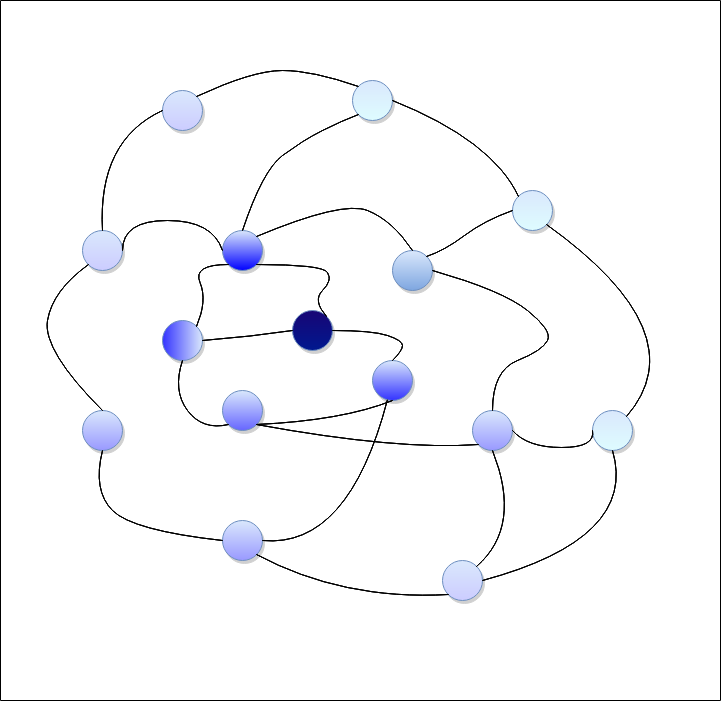
\includegraphics[scale=0.5]{p2p}
	\centering
	\caption{Peer Arrangement}
	\label{fig:p-arrange}
\end{figure}


\begin{algorithm}[h]
\caption{Eventual Leader Selection - Leader} 
\label{leader}
\begin{algorithmic}[1]
\Upon[init]{nodeId}
  \State $selfId := nodeId;$ $round := 0;$
  \State $isLeader := false;$ $stableGradient := false;$
  \State $gradSample := \emptyset;$ $followerGroup := \emptyset;$
  \TriggerS[periodicCheck]{}\EndTriggerS
 \EndUpon

\Upon[gradientSample]{sample}
  \State $stableGradient := $ \emph{stable}$(sample);$
  \State $gradientSample := sample;$
 \EndUpon

\UponS[periodicCheck]{}
  \If{$!isLeader$ AND $stableGradient$ AND \emph{highestUtility}$(selfId, gradientSample)$}
     \State $followerGroup := $ \emph{getTopK}$(gradientSample);$
     \ForEach[followerGroup]{member}
       \Trigger[promiseReq]{selfId, round} \EndTrigger
    \EndForEach
    \TriggerS[roundTimeout]{} \EndTriggerS
    \State $promiseSet := \emptyset$
  \EndIf
 \EndUponS

\Upon[promiseAck]{pNodeId, pRound}
  \If{pRound = round}
    \State $promiseSet := promiseSet \cup \{pNodeId\}$
    \If{followerGroup = promiseSet}
      \ForEach[followerGroup]{member}
        \Trigger[lease]{selfId}\EndTrigger 
      \EndForEach
      \State $isLeader := true;$
      \TriggerS[leaseTimeout]{}\EndTriggerS
      \TriggerS[cancelRoundTimeout]{}\EndTriggerS
    \EndIf
  \EndIf
\EndUpon

\Upon[promiseNack]{pNodeId, pRound} 
  \If{pRound = round}
    \State $round++;$
    \TriggerS[cancelRoundTimeout]{}\EndTriggerS
  \EndIf
\EndUpon

\UponS[roundTimeout]{}
  \State $round++$
\EndUponS

\UponS[leaseTimeout]{} 
  \State $sample := $ \emph{resetUtility}$(gradientSample);$
  \If{\emph{highestUtility}$(sample)$}
    \State $followerGroup := $ \emph{getTopK}$(sample)$
    \ForEach[followerGroup]{member}
      \Trigger[lease]{nodeId} \EndTrigger
    \EndForEach
    \TriggerS[leaseTimeout]{}\EndTriggerS
  \Else
    \State $isLeader := false;$
  \EndIf
\EndUponS

\end{algorithmic}
\end{algorithm}

\begin{algorithm}[h]
\caption{Eventual Leader Selection - Follower} 
\label{follower}
\begin{algorithmic}[1]

\UponS[init]{id}
  \State $isFolower := false;$
  \State $selfId := Id;$ $pendingPromise := Nil;$
  \State $gradientSample := \emptyset;$
\EndUponS

\Upon[gradientSample]{sample}
  \State $gradientSample := sample;$
 \EndUpon

\Upon[promiseReq]{nodeId, round}
  \If{$!isFollower$ AND $pendingPromise = Nil$ AND \emph{highestUtility}$(nodeId, gradientSample)$}
    \State $pendingPromise := nodeId;$
    \Trigger[promiseAck]{selfId, round}\EndTrigger
    \TriggerS[promiseTimeout]{}\EndTriggerS
  \Else
     \Trigger[promiseNack]{selfId, round}\EndTrigger
  \EndIf
\EndUpon

\UponS[promiseTimeout]{}
  \State $pendingPromise := Nil;$
\EndUponS

\Upon[lease]{nodeId} 
  \If{$pendingPromise = nodeId $}
    \TriggerS[followerLeaseTimeout]{}\EndTriggerS
    \TriggerS[cancelPromiseTimeout]{}\EndTriggerS
    \State $isFollower := true;$
    \State \emph{setFollowerUtility}$();$
  \EndIf
\EndUpon

\UponS[promiseTimeout]{}
  \State $pendingPromise := Nil;$
\EndUponS

\UponS[leaseTimeout]{} 
  \State $isFollower := false;$
  \State \emph{resetFollowerUtility}$();$
\EndUponS

\end{algorithmic}
\end{algorithm}







\subsection{Preference and Utility Function}

Each peer in the system has an associated utility based on the state of the peer at that instant. As the system evolves with time, so does its utility. As already mentioned, in order to build the overlay network, system uses a \textit {Preference Function} based on the utilities of the nodes. A peer uses this preference function mainly during the selection of peer for shuffling and to keep track of preferred neighbors. The preference function in case of  Sweep is selection of the peers which have a higher utility than self but closer to self with higher probability. As seen in the diagram, if we assume utility having an absolute value, as per the preference function, \textit{Peer C} will prefer \textit{Peer A} over \textit{Peer B}, even though both have higher utility than C because A's utility is closer to utility of A.

\par The preference function is based on the utility of a particular peer. It helps a peer to select a preferred peer from a collection of peers. The utility function is generally any metric or set of rules usually depending upon the application requirement which would help to create a total order on the peers in the system. In case of Sweep, the utility function is as follows:

\small 
\begin{equation*}
    LeaderGroup \prec ReplicationScore \prec PeerScore \prec PeerID
\end{equation*}
\normalsize

In process of comparison of utility values between two different nodes, we simply compare them in order defined above i.e from \textit {left to right}. We move on to the next parameter in the utility function in case ordering cannot be achieved on the previous parameter. The utility function comparison starts by looking at the leader group membership check which indicates if a node is part of leader group for a particular shard. In case a node has this check switched on, the utility of the node suddenly increases compared to the other peers in the same shard. The Replication Score parameter indicates the quantity of the entries that a peer has its local lucene store. As system evolves and more entries are added in the shard the peer with a higher \textit{Replication Score} count indicates a better node in terms of serving latest entries added. Keeping in view the fairness protocol, we also have a \textit{PeerScore} metric in the utility function. This score helps to identify the peers with superior resources in terms of computational capability, higher bandwidth. These nodes are given importance as they can easily serve a larger audience in the shard. The peer id is used a tie breaker in the function. We assume that the peers joining the system have unique peer id's.  In this way, we achieve a total order on the peers in the system.

\par The benefit of achieveing total order on the nodes is the ability to assign ranks to the nodes with the lowest rank i.e. 0 being assigned to the \textit{leader} of the shard. As the system is continously evolving, the utility of peers is changing and therefore the peers in the shard based on the neighboring peers can then adjust there own ranks. The purpose of assigning ranks is the creation of fingers which are nothing but long range links that each peer hold. Based on the rank, the peer usually try to find fingers i.e. links to the peers that are half its own rank. These fingers help speeding up the dissemination of the updates in the system.


\subsection{Pull Protocol}

The general overall functioning of the system involves electing a leader i.e a node with the highest utility at that instant of time as the leader of shard. The leader takes decisions in the shard in terms of addition/ deletion and updating entries in the shard. In order to prevent a single point of failure the leader performs a two phase commit to the nodes elected as part of leader group. The Leader Election protocol is explained later in detail in section [mention section]. Once the entry has been replicated to the leader group nodes, the leader returns back a successful response to the client. Now the peers can either push the entries to the neighboring nodes or nodes need to pull the entries added. The push protocol seems lucrative in terms that the peers as soon as they discover about a new entry, push the entry to other nodes. It prevents the other nodes constantly looking for the entries by asking the higher utility nodes. But there are major flaws in this scheme.

\begin{enumerate}

\item First, we cannot guarantee that the entry will be received by every node in the shard as it is based on push protocol and current neighbors. In case a particular peers reference is not in the higher utility nodes, the entry will not be pushed to it.

\item It makes the system vulnerable to Byzantine Nodes [reference] which can easily push junk data.

\item The biggest flaw in this protocol is way in which the preference function is defined. As mentioned earlier a particular node prefers node which higher but closer utility. This means that given enough peers which have higher utility, the peers neighbors will all point to the nodes above in the Gradient, therefore the nodes which are on the edges of a particular shard will never receive the entry.

\end{enumerate} 

As a result, we introduced pull protocol, in which the nodes constantly request the peers higher than self in terms of utility about any latest developments or decisions taken in the shard by the leader. This way there are able to disseminate the information in the system. The dissemination protocol will be explained in greater detail in section [mention section]



\subsection{Gossip Based Data Dissemination}
Once a peer becomes a leader, it is implicitly trusted by other members in the shard.
Initially the information of a node becoming a leader is only published at the leader group chosen by the leader. This information then gets pulled by other peers in the system. In this situation, it might be very much possible that a Byzantine Node might start publishing wrong information to the peers during the pull protocol. In order to avoid such situations, a peer during the pull protocol, requests updates from a predefined configurable peers usually three that are above itself in terms of utility.  The peers respond with the hashes of the information. Only the information for which the hashes match from all the nodes is then pulled from anyone of the responding peers. 
\par This approach is being used for securely disseminating the leader information in the system. In addition to this, entry dissemination is also based on this protocol. We think that this approach is secure enough in the sense that it is highly unlikely for all the nodes that are requested by peer to provide updates to be faulty.


\subsection{Load Balancing}

As the system evolves, the leader receives request for adding new entries in the system. Using basic replication strategies the leader commits the entries to the leader group which then gets replicated to all the nodes in the shard using pull protocol. The system has a predefined \textit{MaxShardSize} parameter. When the entries grow beyond the count, the leader then initiates \textit{ShardSplit} protocol. As part of this protocol, each peer based on its identifier and its depth which is basically number of shard splits seen by the node, decides the next shard id. 
\par Before initiating the two phase commit of the shard split, the leader stops handling the entry additions. It then looks in its local lucene store and after sorting the entries based on there identifiers, calculates the split point. This meta information is then committed to the leader group nodes along with the shard split update as a part of two phase commit. Once the information is pulled by other peers in the system, based on there new shardId, they decide to remove all the entries either before or after the split point. The peers then join the other peers in there respective shards. 
\par It might be argued that after the shard split, the entries get divided, so the search results might not be complete. It order to prevent this, each peer has a \textit{routing table} which keeps references to the peers in other shards. The table gets populated and updated by our \textit{Peer Sampling Service} which provides peers with random samples from different shards. Upon receiving shard request, the peer simply forwards the request to the peers in the other shards.


\subsection{Large Fanout}
In this section, we will be discussing the concept of \textit{latency variability} in large scale distributed systems. The term latency variability means the distribution of latencies during an operation over the network. The importance of latency variability has increased in recent times due to the requirement for real time responsiveness of applications. Google quickly discovered that simply scaling the system doesn't necessarily means better performance during the response times of search requests[reference taming]. This is due to the presence of a long tail. Normally the requests handled by a particular server are within the limits of respectable response times but once in a while the response time for a request would be much higher. This may be attributed to the network beign slow due to choke or system disk from which the data is supposed to be read is acting slow. This phenomenon of long tail has also been observed in trading systems where we might find the latencies of few trades in order of 900ms compared to normal latency of 5ms. 

\par We might argue that the occurence of the phenomenon is not often enough to cause alarm but as the scale of the system keeps on growing as in case of Google where the data is divided into multiple shards. Now the search request needs to be faned out to a larger audience and therefore the probability of occurence of long tail increases as the requesting node needs to wait for responses from all the shards. This leads to unacceptable response times occuring with higher probability. 

\par Google uses a lot of inovative approaches to solve issue of latency variability as mentioned by Jeffery Dean in this talk[reference jeff dean]. The approach that we are interested and have adapted for our prototype involves instead of sending to a single node in every shard the search request, we send it to a predefined number of nodes in that shard. We simply wait for the first response from that shard and discard the rest. The purpose behind it is to reduce the dependency on the slow performing node by replicating the request to other nodes within the same shard. Once all the shards have responded or search timed out, we collect, filter and augment the results with some metadata. This data is then returned to the requesting node. In this way the system makes significant steps towards preventing long tail in the response times during the search request.

\begin{itemize}

\item Application Entries.

\end{itemize}


\section{Network Partition Merge}

\subsection{Entry Identifier Structure}
The structure of the identifier used by the system to handle the entries is mainly composed of three parts. 

\begin{tcolorbox}
Epoch Structure: \textless Epoch, LeaderId, EntryId \textgreater
\end{tcolorbox}

The epoch is simply a counter which a peer when elected as the leader checks the epoch of the previous leader, increments it and then starts adding the entries in the system with the updated epoch. The second component i.e. leaderid is simply the node identifier which the peer joins the system. An invariant that we maintain is that in a system is that each peer joins the system with a different identifier. Therefore at any given time in the system, there won't be any two nodes with the same  identifier. The reason behind the invariant is that the identifier of the node act as tie breaker in the preference function used to provide total ordering on the nodes.

\par Each leader starts committing the entries with a predefined starting value of the entry id which gets incremented on every subsequent entry add. The main reason behind using this identifier structure is to enable creation of dense spaces. The epoch identifier helps the system to evolve and move forward.


\subsection{Leader Unit}
A collection of entries added by a leader in a particular epoch is termed as a \textit{leader unit}. Each leader within a particular epoch can add only a predefined amount of entries. As the number of entries reaches the threshold, the leader needs to perform a mandatory epoch switch. 

\begin{tcolorbox}
Leader Unit Structure: \textless Epoch, LeaderId, MaxEntries \textgreater
\end{tcolorbox}

\subsection{Marker Entry}
Before a leader can start committing entries in a particular epoch, it needs to inform the other nodes in the shard about the epoch switchd. The leader needs to make a \textit{marker entry} commit which will indicate the other nodes about the starting of the new epoch. The marker entry commit contains the maximum number of entries added by the previous leader. The current leader analyzes in its data storage module to calculate the entries added in the previous epoch. This information is committed to the leader group nodes which gets propagated to the system through the pull protocol.

\subsection{Timeline}
As the system is dynamic any node can join and leave the system. In case the system has evolved enough and a new node joins the system, the new nodes also needs to pull entries from the neighbouring nodes and evolve in the same manner to reach the stage at which the other nodes are present. Therefore the other nodes needs to keep track of the leader unit history. The timeline is an abstraction which mainly keeps track of the evolution of the system in terms of leader units added. Whenever a new leader unit switch happens, the update needs to happen in the timeline regrading the previous and current leader units. In addition to this, the timeline also keeps track of the current leader unit being pulled by a node and identify the next leader units based on the current unit which is used during the control pull requiring the next leader units added in the system.

\par In order for the timeline to function correctly, an invariant that we maintain is that a node will not add a leader unit out of order, meaning that the leader units will always be added in the timeline based on increasing epochs. In case a jump is seen in the  epoch identifier, the leader unit is buffered till the in order leader units are pulled.
The reason behind maintaining this invariant is to prevent creation of entry gaps.


\chapter{Implementation}
\label{sec:impl}

In order to check for the viability of the theoretical approach we worked on developing a prototype on the principles stated in the design section. The prototype used Apache Lucene for storing and indexing data. In addition to this, the prototype was developed using the Kompics which is an asynchronous message passing system. The main sweep process on each node in the system is composed of following abstractions: \textit {group membership, routing, leader election} and \textit{data storage} abstraction . All the modules interact with the \textit{network} and \textit{timer} abstraction which are used to send messages over UDP and configure local timeouts respectively. In addition to this, we have a \textit{message chunking} abstraction which as name suggests check the messages going over the network and in case the message exceeds the max transmission limit, fragments the packet and at the receiving end joins the fragments to construct the final message. All the abstractions are built from scratch in Java.
\par The main application module interacts with the above mentioned abstractions. It is responsible for \textit{Indexing} and \textit{Searching} of the documents in the system. In case a node receives a request for adding an entry in the system, the module firstly check whether the node is the leader for the current shard. In case it is the leader, it invokes the entry addition routine on self. Otherwise, it sends the request to the routing module to route the request to the leader. As part of current implementation, the entry addition routine is a synchronous operation which involves performing a two phase commit by the leader over the leader group nodes. In order to commit the entry the application module interacts with the data module to perform add the entry in the lucene. Once the entry gets replicated, the leader responds back to the node on which the request originated. 
\par As part of searching for entries, the user enters the name of the document to be located. The middleware constructs a well defined search pattern which the lucene in the data storage abstraction understands. The search request is initially handled by the application module of the client. The application module sends this request to the routing module to check for the references of the nodes located in different shards in the system which are populated by the gossiping protocol constantly pushing subset of the global samples to the routing module. The module then routes the request to the nodes in each shard. As the number of shards can grow therefore, it can easily result in large fanout search causing a long tail. To prevent this, we route request to more than one node in each shard and only handle the response from the fastest node and reject the other responses. The search responses are added in a separate lucene instance. In case all the shards responded or the timeout for search whichever gets triggered first, the responses are then sorted and returned back to the client. 

\subsection{Overlay Network}
The system strives to be a dynamic system in which the nodes can join and leave depending upon there requirement. Gradient Topology over peer sampling service is being used to construct the overlay. As already mentioned, each peer holds references to limited number of other peers in the system. Now as the node leaves the system voluntarily or by crashing, the sample becomes stale. As an effort to keep neighborhood samples fresh, in case the size of the sample list grew beyond a predefined threshold we removed the oldest sample i.e peer reference with the highest age. We quickly realized that if this approach needs to be successful, we would need to synchronize the rate at which the gradient and the peer sampling service performs shuffling with the neighborhood nodes.
\par In case the difference between the shuffling rates of both the services is large, the outcomes of the stabilization of the gradient were unexpected. The main reason behind it is that the peer sampling service feeds the sample to the gradient service. So in case the rate of shuffling in the croupier is fast, the increment in the ages would be frequent because as part of shuffling the peers increment the age of the references and then exchange sample. Therefore the croupier will feed the samples with high ages and the gradient shuffling is at a lower rate resulting in the slow rate of increase in ages. The nodes disseminate there updated utility in the system through the shuffles. Therefore, the probability of peer reference samples having ages higher than the corresponding samples present in the gradient sample is higher even though the reference from the sampling service has updated utility. It is because of the large gap in the shuffling rates of the both the services. Thus, the updated peer reference sample gets disseminated in the system slowly.

\subsection{Operations}
As part of current implementation, the \textit{Sweep} prototype supports the following operations:

\begin{itemize}

\item \textit{add-entry (name, category, desc, date)}
\item \textit{search-entry (name)}

\end{itemize}




\chapter{Evaluations}
\label{sec:eval}

In this section we will be writing about the various experiments that were performed.

\section{Experimental Setup}

The evaluations were performed on the machine with the following specifications:

\begin{itemize}

\item 8GB of RAM
\item Eight Cores (Intel(R) Core(TM) i7 CPU 860  @ 2.80GHz)
\end{itemize}

The nodes were started in simulation on a single machine. A helper module was used to keep track of all the nodes started in simulation in order to communicate with them during the entry addition phase. A special node known as the leader node was also started with the lowest value of the identifier. Keeping other parameters as same, this allowed the node to become leader during the initial leader election phase. In addition to this, a global aggregator node was also booted. The peers internally have a local aggregator component which keeps track of the overall state of the peer based on the information received from various other components. The local aggregator constantly sends the information over to the global aggregator node. In this we are able to keep track of the overall state of the system.



\section{Workload Setup}

Unless otherwise specifically mentioned, we ran simulations with cluster of 200 nodes. The simulation in Kompics is single threaded in order to reproduce the results, the limiting factor was the capacity of single core of the machine. The other parameters that were tuned for the simulations are as follows:

\begin{itemize}
\setlength\itemsep{0em}
\item \textit{gradientViewSize} - 10 nodes
\item \textit{croupierViewSize} - 10 nodes
\item \textit{gradientShuffle} - 1000 (ms)
\item \textit{croupierShuffle} - 1000 (ms)
\item \textit{branchingFactor} - 10
\item \textit{electionConvergenceRounds} - 6
\item \textit{electionConvergenceTest} - 0.8d
\item \textit{Entry Pull Round} - 4000 (ms)
\item \textit{Control Pull Round} - 3000 (ms)
\item \textit{maxEntryExchange} - 25 nodes/ pull
\end{itemize}

In addition to it, the minimum nodes that nodes needs to pull either control or the entry data needs to be \textbf{three}. This conditions is respected by each and every node unless they find the leader in the view of there own gradient. Every node implicitly trusts the leader and therefore pull data directly from it.




\section{Convergence Experiment}

The \textit{Convergence Experiment} helps to understands the rapidness with which the entry gets disseminated in the system. As part of this experiment, we booted up 250 nodes in simulation. Once the system was stabilized in terms of leader of the shard getting elected and the marker entry for the current epoch was already added to each node, we then added a single entry to the leader and analyzed the time it took for the entry to be disseminated to all the nodes in the system. The results as shown in Figure \ref{fig:250conv} points out that it took 8 - 9 (sec) for all the nodes to get the entry. This time evaluates to roughly two pull rounds based on the current pull round timeout.

\begin{figure}[h]
	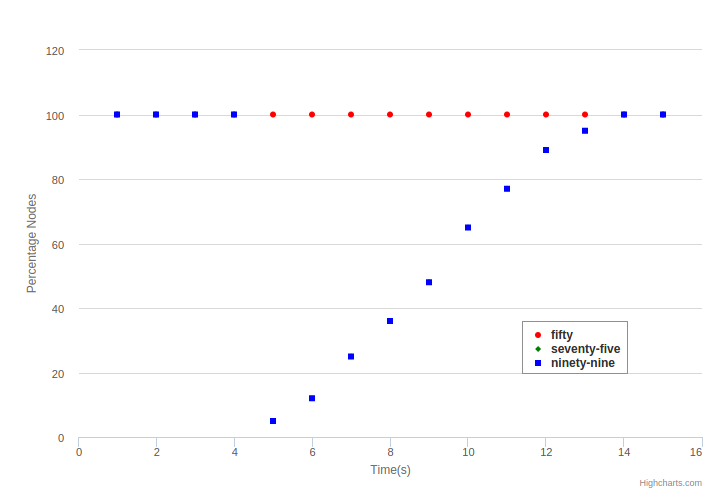
\includegraphics[scale=0.5]{250Convergence}
	\caption{Convergence - 250 nodes}
	\label{fig:250conv}
\end{figure}


Figure \ref{fig:500conv} shows the same experiment but now with 500 nodes in the simulation. The outcome is same as the previous one. The reason is because of the \textit{branchingFactor} parameter which is set to 10. Because of this, the nodes in the range of 60-600 are supposed to get the entry in approx 2 rounds. The results also conform with the expected outcome. 


\begin{figure}[h]
	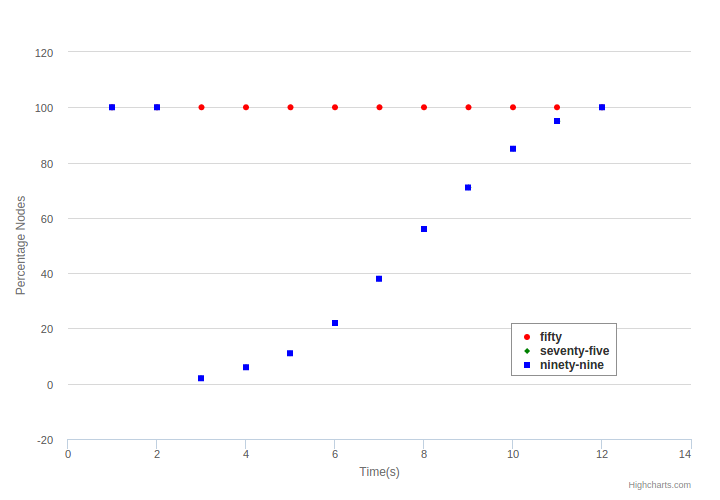
\includegraphics[scale=0.5]{500Convergence}
	\caption{Convergence - 500 nodes}
	\label{fig:500conv}
\end{figure}


\section{Add Entry Throughput}

In this experiment, we initially booted up 200 nodes in simulation. Once the gradient and the leader group becomes stabilized, initial batch of 20 entries were added in the system. We then started adding entries at varying rates likes \textit{1 entry per sec}, \textit{2 entry per sec} and  \textit{6 entry per sec} for a fixed predefined period of time. As part of this experiment, we analyzed the fifty, seventy five and ninety nine percentile values i.e. number of nodes which at any given time during the operation of entry addition have fifty percent, seventy five percent and ninety nine percent of the entries. 

\par The Figure \ref{fig:addEntry1} depicts the metrics in case of \textit{1 entry per sec}. As we can see the fifty percentile metrics seems stable as in all the nodes during the entry addition phase has atleast fifty percent or more of the entries. In case of seventy five percentile, it depicts a seesaw like structure. This behavior of the system initially looks strange but a closer look at the interaction of the application with the overlay over which the system is built can help to understand this behavior. As mentioned earlier, a node in order to perform a control pull needs to have atleast three nodes above himself in terms of utility. The node then matches the responses and incorporate the common in order responses in the local \textit{timeline}. As node mainly fetches the leader unit updates through the control pull, the entry pull mechanism takes this updated information about the number of entries in the system, requests for the next entries from the nodes above it. The mechanism of matching the responses is same as in case of control pull protocol. 

\begin{figure}[h]
	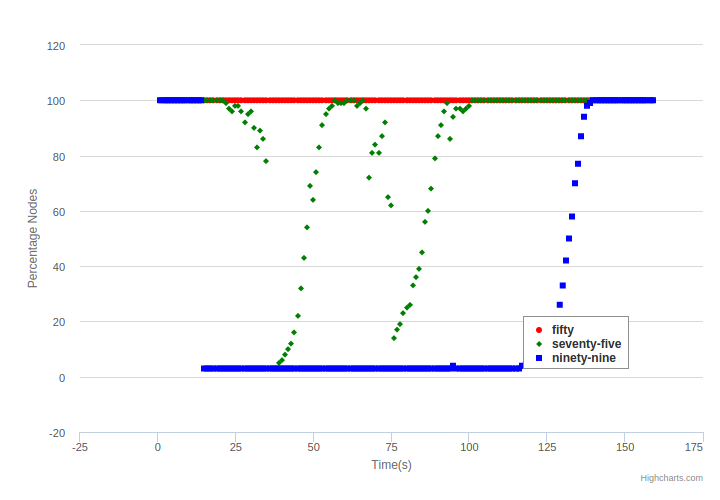
\includegraphics[scale=0.5]{200-1EntryPerSec}
	\caption{Add-Entry 1 entry(s)/Sec}
	\label{fig:addEntry1}
\end{figure}

\par The node then incorporates the entries by adding them to the Lucene Store and augmenting the utility accordingly. The application then informs the other components about its updated utility which allows them to make informed decisions. The overlay network contains the sample of nodes based on the preference function. With a sudden increase in the utility the local view of the gradient becomes obsolete and therefore the number higher samples return by the gradient to the application diminish. In case a node unable to find desired number of higher utility nodes for the control pull simply returns. It is because of the obsolete gradient samples the node doesn't start the control pull. In absence of the updated information about the entries in the system, the entry pull mechanism is unable to pull the next entries. Therefore the nodes in range of seventy percentile drops. Once the sample gets refreshed due to continuous shuffling and nodes injecting updated utilities in the system, the nodes are able to find the nodes above itself and start pulling the control information  resulting in the new entries being pulled.

\par Figure \ref{fig:addEntry6} depicts the performance of the system in event of addition of \textit{6 entry per sec}. The seesaw like structure can now be observed both in the fifty and seventy-five percentile. The reason being same as mentioned above. As the nodes near to the center of the gradient waits for the gradient to stabilize to get updated information, the nodes farther away near to the edges of the gradient are also unable to get the updated information. Thus they also start lagging in terms of catching up to the leader group with has the latest information in terms of entries being added in the system. Apart from this, as observed from the diagrams the ninety percentile is really low in range of \textit{1-3\%}. The reason for this is the entries present in the system. As the entries that are added are usually low in addition to the initial entries, even a difference of one entry will remove a particular node from the ninety percentile. Therefore only the leader group nodes to which the leader replicates the entry are present in this range.

\begin{figure}[h]
	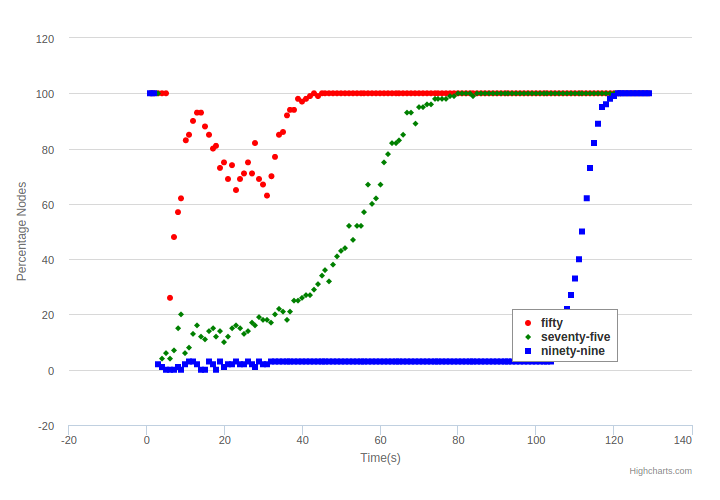
\includegraphics[scale=0.5]{200-6EntryPerSec}
	\caption{Add-Entry 6 entries/Sec}
	\label{fig:addEntry6}
\end{figure}

\section{Churn Experiment}

As part of this experiment, we initially started the system with 200 nodes and loaded the system with 100 entries. We started with the addition and the simultaneous removal \textit{4 Nodes per sec} of the node from the system. We continued this behavior for \textit{60 Seconds} thus resulting in a churn of \textit{4 \%}. Nodes from the system except the nodes from the leader group were selected randomly to be removed by stopping there execution. New nodes were booted up with different node ids. In addition to this, a constant rate of \textit{1 entry per sec} was employed for the entry addition. Figure \ref{fig:churn} depicts the fifty, seventy five and the ninety percentile values. As we can see more than fifty percent of the nodes had fifty and seventy percent of the entries at all times during the experiment. Only the leader group nodes seemed to be in the category of nodes having ninety nine percent of the entries at all times. 

\begin{figure}[h]
	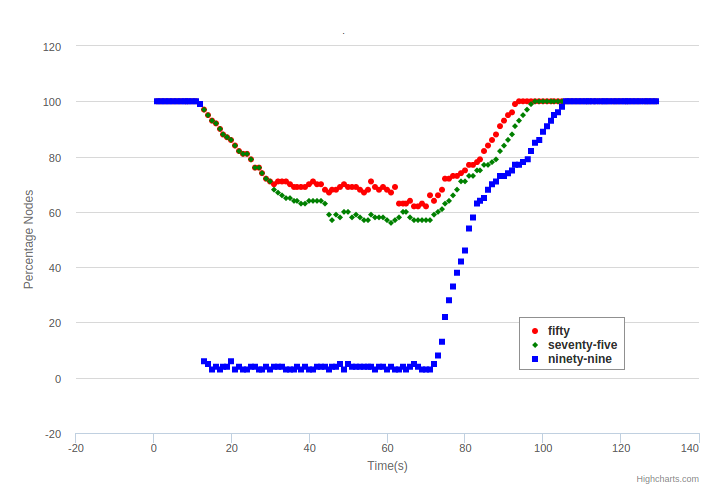
\includegraphics[scale=0.5]{200-4Node-1Entry}
	\caption{Churn 4 nodes/sec and 1 entry/sec}
	\label{fig:churn}
\end{figure}

\section{Flash Crowd Experiment}
As part of this experiment we started with 200 nodes in the system and loaded the system initially with 100 entries. Then we introduced bunch of fresh nodes in the system simultaneously and analyzed the time it took for the nodes to catch up. We performed the experiment for flash crowd size of \textit{10 percent, 20 percent and 40 percent} respectively. As seem from Figure \ref{fig:flash40} and \ref{fig:flash80}, it took \textit{20 seconds approximately} for the nodes to catch up with fifty percent of the entries. In addition to this, the time taken by nodes to catch up with the seventy five and ninety nine of the entries is approximately the same. 

\begin{figure}[h]
	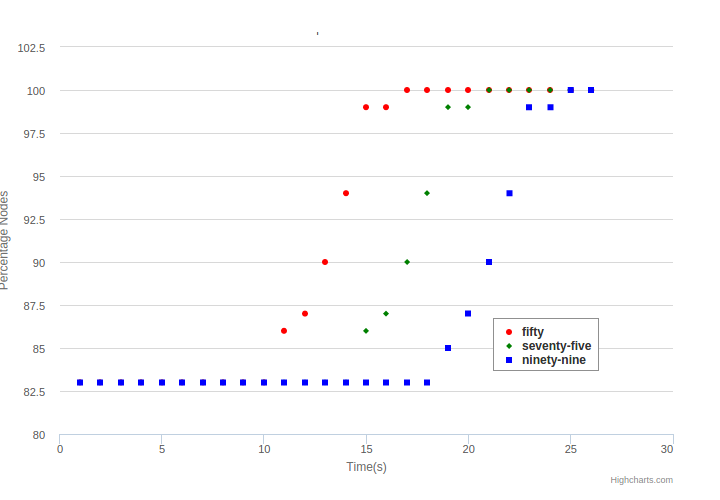
\includegraphics[scale=0.5]{200-40Nodes}
	\caption{FlashCrowd 40 nodes/Sec }
	\label{fig:flash40}
\end{figure}

\par Ideally as the \textit{maxEntryFetch} parameter per entry pull is \textit{twenty five}, it should take sixteen seconds i.e \textit{4 pull rounds} approximately for the nodes to fetch all the entries in the system but as observed from the diagram it takes more time than that. It is because it takes some time for the nodes to adjust themselves in the overall gradient and then pull the control information. Once the control information is pulled and verified, the nodes are able to determine the entries in the system at that moment and then start looking for the entries by requesting them from the nodes higher than themselves in terms of utility.

\begin{figure}[h]
	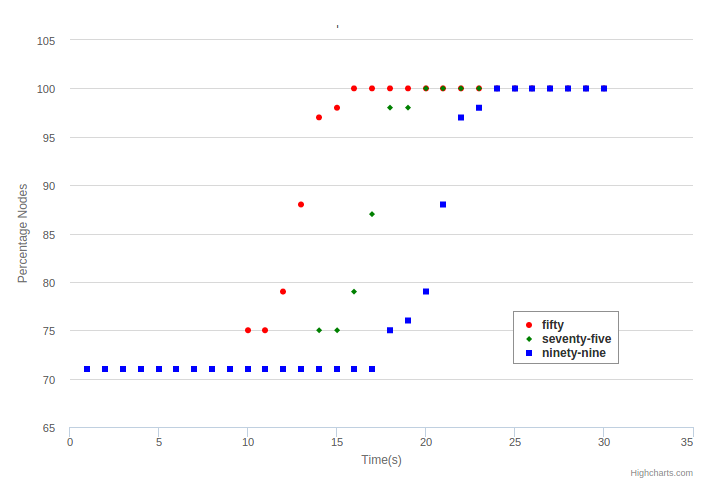
\includegraphics[scale=0.5]{200-80Nodes}
	\caption{FlashCrowd 80 nodes/Sec }
	\label{fig:flash80}
\end{figure}



\chapter{Conclusions}
\label{chap:conclusion}

This chapter explains the conclusions obtained throughout the design,
development, and evaluation described in this thesis and proposes a number of
improvements, extensions, or complements that may be of interest in order to
continue this work. Page filling text mass. Page filling text mass. Page
filling text mass. Page filling text mass. Page filling text mass. Page
filling text mass. Page filling text mass. Page filling text mass. Page
filling text mass. Page filling text mass. Page filling text mass.

\section{Conclusion}
%% Did you meet your goals?
%% What insights have you gained?
%% What suggestions can you give to others working in this area?
%% If you had it to do again, what would you have done differently?


In this section we will state the conclusions and insights gained as result of this thesis project.

\subsection{Goals}
\label{ssec:goals}

The project met five of the ten initial goals. With the third goal not
addressed at all and goals 6-10 only partially met. Page filling text
mass. Page filling text mass. Page filling text mass. Page filling text
mass. Page filling text mass. Page filling text mass. Page filling text
mass. Page filling text mass. Page filling text mass. Page filling text
mass. Page filling text mass.


\subsection{Insights and suggestions for further work}
\label{ssec:insights-and-suggestions}

One of the most important insights to come from this work is the need to
understand the interaction between the IP layer and the link
layer. Unforunately I did not have time to examine this in detail in this
thesis. However, the data shows that paying attendtion to this APR cache
flushing patterns could yield improved performance. Future works should start
by measuring the relationship between the cache validity and number of packets
which are generated at or above the IP layer, but not transmitted on the
network.  Page filling text mass. Page filling text mass. Page filling text
mass. Page filling text mass. Page filling text mass. Page filling text
mass. Page filling text mass. Page filling text mass. Page filling text
mass. Page filling text mass. Page filling text mass.

\section{Future work}
\label{sec:future-work}
%% What you have left undone?
%% What are the next obvious things to be done?
%% What hints can you give to the next person who is going to followup upon your work?


Due to the breadth of the problem, only some of the initial goals have been
met. In these section we will focus on some of the remaining issues that
should be addressed in future work. Page filling text mass. Page filling text
mass. Page filling text mass. Page filling text mass. Page filling text
mass. Page filling text mass. Page filling text mass. Page filling text
mass. Page filling text mass. Page filling text mass. Page filling text mass.

\subsection{What has been left undone?}
\label{what-has-been-left-undone}

The prototype does not address the third requirment, i.e., a yearly
unavailability of less than 3 minutes, this remains an open problem.  Page
filling text mass. Page filling text mass. Page filling text mass. Page
filling text mass. Page filling text mass. Page filling text mass. Page
filling text mass. Page filling text mass. Page filling text mass. Page
filling text mass. Page filling text mass.

\subsubsection{Cost analysis}

The current prototype works, but the performance from a cost perspective makes
this an impractical solution. Future work must reduce the cost of this
solution, to do so a cost analysis needs to first be done. Page filling text
mass. Page filling text mass. Page filling text mass. Page filling text
mass. Page filling text mass. Page filling text mass. Page filling text
mass. Page filling text mass. Page filling text mass. Page filling text
mass. Page filling text mass.

\subsubsection{Security}

A future research effort is needed to address the security holes that results
from using a self-signed certificate. Page filling text mass. Page filling
text mass. Page filling text mass. Page filling text mass. Page filling text
mass. Page filling text mass. Page filling text mass. Page filling text
mass. Page filling text mass. Page filling text mass. Page filling text mass.


\subsection{Next obvious things to be done}

In particular, the author of this thesis wishes to point out xxxxxx remains as
a problem to be solved. Solving this problem is the next thing that should be
done. Page filling text mass. Page filling text mass. Page filling text
mass. Page filling text mass. Page filling text mass. Page filling text
mass. Page filling text mass. Page filling text mass. Page filling text
mass. Page filling text mass. Page filling text mass.

\section{Required Reflections}
\label{sec:req-reflections}


\bibliography{report}
%%\bibliographystyle{IEEEtran}
%%\bibliographystyle{unsrturl}
%%\bibliographystyle{unsrtnat}
\bibliographystyle{myIEEEtran}
\appendix
\chapter{Insensible Approximation}

\backmatter

\end{document}
